% Build: cd examples && TEXINPUTS="../templates/neurips:" latexmk -pdf showcase-neurips.tex
% PNG:   pdftoppm -png -r 150 -singlefile showcase-neurips.pdf showcase-neurips
\documentclass{article}
\usepackage[main,final]{neurips_2026}
\usepackage{graphicx}
\begin{document}

\section*{NeurIPS figure layout examples}

These two figures were generated by \texttt{figspec} for the official
NeurIPS 2026 single-column template. Both are included at their natural
size, without a width argument.

\begin{center}
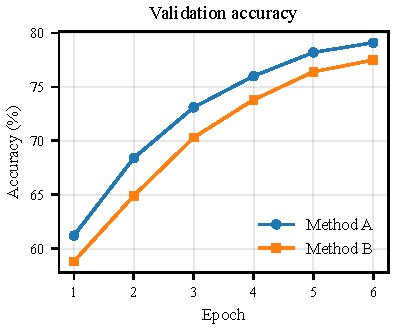
\includegraphics{neurips-single.pdf}
\end{center}

\textbf{Single-column layout.} The figure uses 48\% of the text width
(190.8\,pt, 2.64\,in). Labels and legends are 8\,pt, ticks 7\,pt, and
panel titles 9\,pt.

\begin{center}
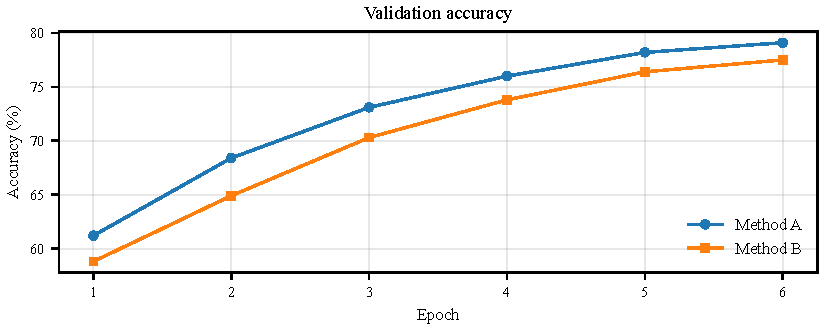
\includegraphics{neurips-double.pdf}
\end{center}

\textbf{Double-column layout.} The figure uses the full text width
(397.5\,pt, 5.50\,in), with the same font hierarchy. Both PDFs are at their
final size; no scaling is applied when they are included.

\end{document}
